\subsection{Epidemiologia}
L'epidemiologia è la disciplina biomedica che studia la 
distribuzione e la frequenza delle malattie ed eventi di 
rilevanza sanitaria nella popolazione \cite{wiki:Epidemiologia}.
Si occupa di analizzare le cause, il decorso e le 
conseguenze delle malattie.

\cite{Galea2009-lj} \cite{Parascandola2001-kw}

\subsubsection{Causalità in Epidemiologia}
L'epidemiologia è una disciplina molto pratica, che visto 
l'obiettivo che si pone, quello di trovare le cause
relative ad un dato effetto, non può esentarsi dagli 
svariati problemi che gravitano e definiscono questo 
nobile obiettivo, primo tra tutti: cosa vuol dire che un
evento è causa di un altro? e come definisco questo 
tipo di rapporto in maniera inequivocabile?

Questi interrogativi possono sembrare banali in quanto 
come specie ci siamo evoluti per trovare una correlazione
di causalità tra eventi anche quando questi non ne hanno.
Ad esempio se fossimo in un bosco, al buio e soli con
l'unico rumore ad accompagnarci che è quello di una 
piacevole brezza estiva, se percepissimo un rumore tra 
i cespugli, molto probabilmente penseremmo che c'è 
qualcosa che non va, che ci sia un pericolo in agguato, 
anche se magari la motivazione è la suddetta brezza. 

Questo adattamento evolutivo ci ha permeso di sopravvivere
in situazioni di pericolo, ma sfortunatamente quando 
si parla di scienza e di dati, non sempre l'istinto è qualcosa 
a cui affidarsi. 

\begin{figure}[h]
    \begin{center}
        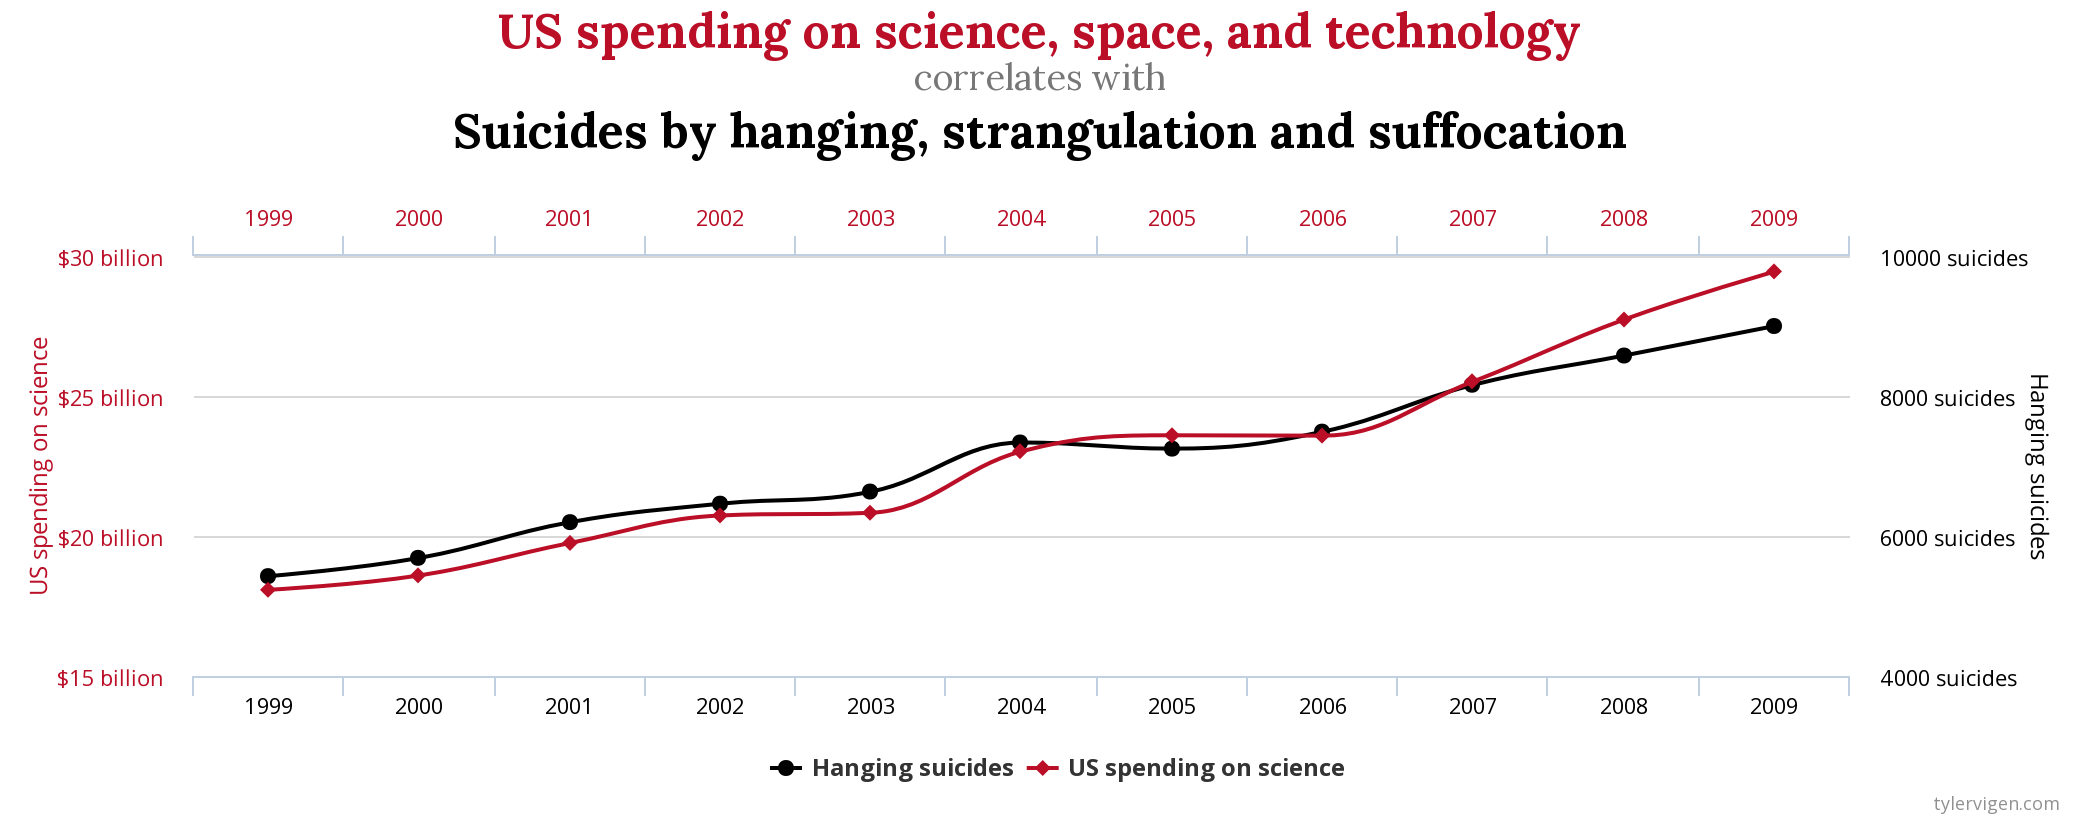
\includegraphics[width=\linewidth]{img/chart.png}
        \caption{Esempio di correlazione spuria da \url{https://www.tylervigen.com/spurious-correlations}}
        \label{fig:spurious_relations}
    \end{center}
\end{figure}

Affidandoci solamente al grafico e ai dati riportati in figura, 
ci verrebbbe da pensare che le due categorie siano in qualche
modo correlate, e che il governo americano debba essere fermato, 
in quanto respondabile di incitamento al suicidio.
Ebbene non è così, questo è un caso di relazione spuria \cite{wiki:Spurious_relationship},
ovvero che due o più variabili sono associate ma non causalmente correlate.

E' chiaro quindi che non sia così semplice comprendere le cause 
di un determinato effetto, o insieme di effetti. Alle volte
le cause sono completamente contro intuitive e auto alimentanti \cite{wiki:Positive_feedback}, 
il che rende ancora più difficile la loro determinazione.
Altre volte invece le cause dipendono dalle interazioni che hanno 
gli individui tra loro e per cui sono mutevoli in base al 
comportamento degli individui, rendendo pressocchè impossibile
determinare con precisione la causa ma al più è possibile
restringere la propria ricerca ad un insieme minimale di esse \cite{Galea2009-lj}. 

Il problema della causalità quindi non è da prendere sotto 
gamba, ed è uno dei problemi cardine da comprendere quando 
si vogliono determinare e applicare degli interventi all'interno 
di una popolazione per cercare di mitigare la diffusione di
un agente patogeno \cite{Parascandola2001-kw}. Conoscere
l'agente patogeno, o quanto meno la sua natura può aiutare,
ma non sempre è sufficiente. l'utilizzo di modelli di 
Machine Learning per l'estrapolazione di dati, di correlazioni
e successivamente per la definizione di policy di intervento
può risultare in un rischio non indifferente se dovesse succedere
di confondere una relazione spuria con una relazione causale.

Questa confusione sembra impossibile, ma avendo sotto mano
solamente un grande insieme di dati, e una formula che ne descrive
il comportamento, definire con certezza la relazione 
o la non relazione che esiste tra questi è certamente un 
compito arduo e delicato. Tuttavia avere un aiutante in grado 
di analizzare ed estrapolare relazioni da una mole molto 
grande di dati in poco tempo può essere l'aiuto necessario 
per comprendere più velocemente e reattivamente le 
relazioni reali che ci sono tra i dati, arrivando quindi 
a definire delle policy di intervento che sono, al meglio 
delle proprie conoscenze attuali, prive di correlazioni spurie.

\begin{figure}[h]
    \begin{center}
        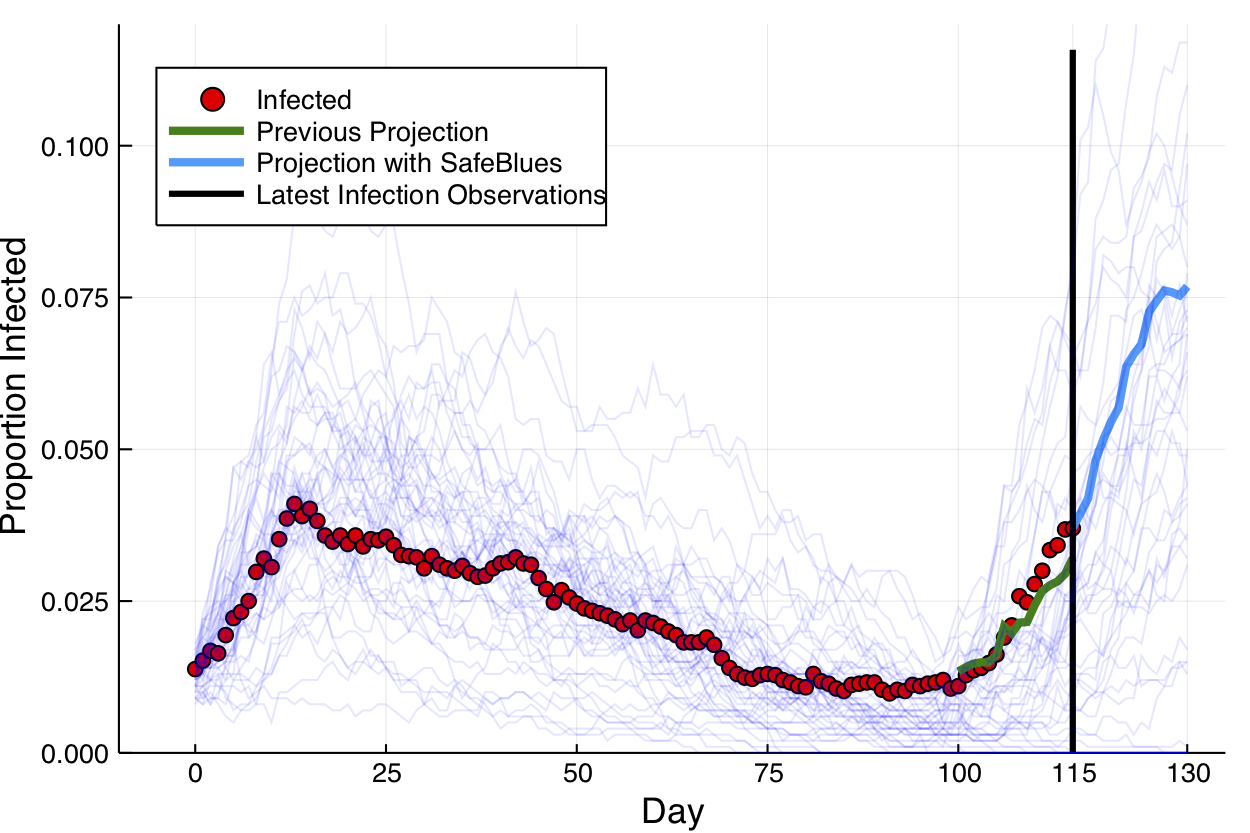
\includegraphics[width=\linewidth]{img/fig1b.png}
        \caption{Esempio di proiezione e previsione dati tramite SafeBlues}
        \label{fig:data_prediction}
    \end{center}
\end{figure}